\subsection{Administrar BBDD (Módulo Administrador principal)}

  \paragraph{}El diagrama de la figura
  \ref{diagramaDescomposicionAdministrarBBDD} representa la estructura del
  módulo Administrar BBDD para el usuario administrador principal. Desde este
  módulo se tendrá acceso a las funciones que se encargan de mantener las tablas
  de la base de datos en las que se almacena la información referente a los
  centros, departamentos, titulaciones, asignaturas, usuarios del sistema y
  a las plantillas de entrevista oficiales.

  \begin{figure}[!ht]
    \begin{center}
      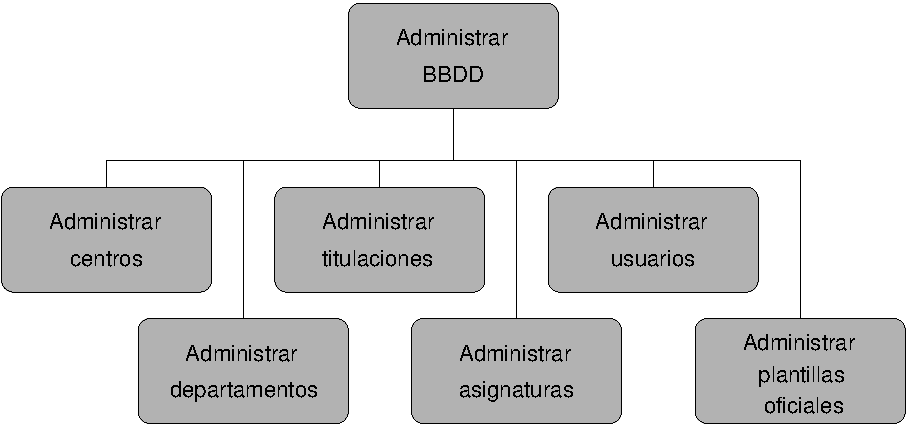
\includegraphics[]{11.Disenyo_Arquitectonico/11.2.Diagramas_Descomposicion/11.2.2.Modulo_administrador_principal/AdministrarBBDD/Diagramas/administrar_bbdd.pdf}
      \caption{Diagrama de descomposición Administrar BBDD (módulo Administrador principal).}
      \label{diagramaDescomposicionAdministrarBBDD}
    \end{center}
  \end{figure}

\subsubsection{Administrar centros (Módulo Administrador principal)}

  \paragraph{}El diagrama de la figura
  \ref{diagramaDescomposicionAdministrarCentros} muestra la estructura del módulo
  Administrar Centros. Este módulo permitirá al usuario administrador principal
  realizar el mantenimiento y gestión de la información relacionada con los
  centros que formen parte del sistema.


  \begin{figure}[!ht]
    \begin{center}
      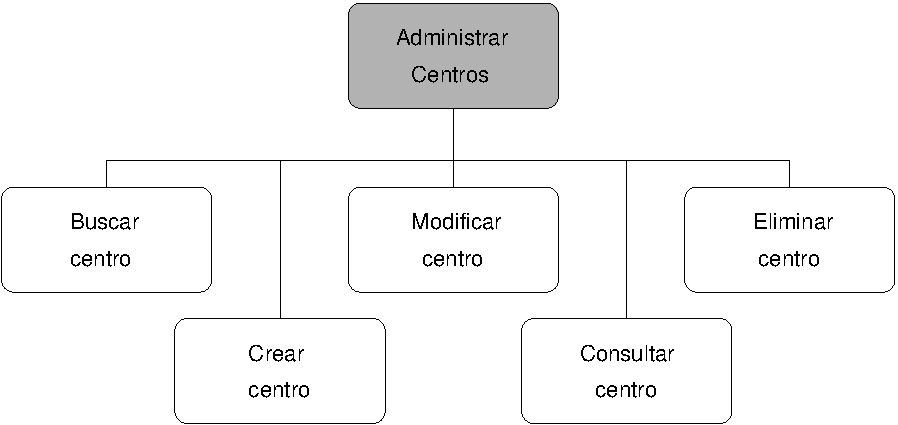
\includegraphics[]{11.Disenyo_Arquitectonico/11.2.Diagramas_Descomposicion/11.2.2.Modulo_administrador_principal/AdministrarBBDD/AdministrarCentros/Diagramas/administrar_centros.pdf}
      \caption{Diagrama de descomposición Administrar Centros (módulo Administrador principal).}
      \label{diagramaDescomposicionAdministrarCentros}
    \end{center}
  \end{figure}

\paragraph{}En este proceso, el usuario administrador principal puede crear,
consultar, modificar o borrar departamentos de la aplicación.

\paragraph{}La figura \ref{diagramaNivel4-AdministrarDepartamentos}
muestra el nivel de abstracción 4: Administrar departamentos.

  \begin{figure}[!ht]
    \begin{center}
      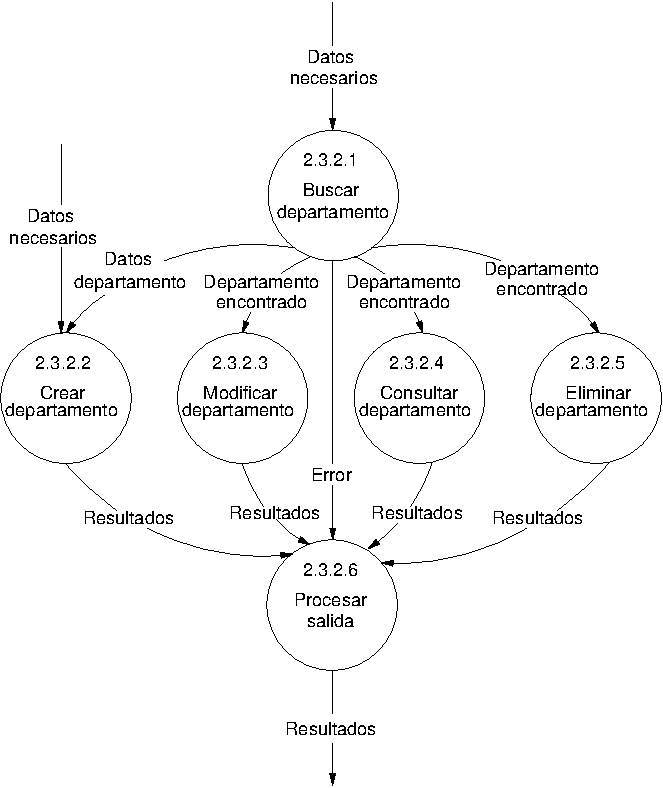
\includegraphics[]{08.Analisis_Funcional/8.2.DFDs/Niveles/Nivel4/AdministradorPrincipal/AdministrarDepartamentos/Diagramas/nivel4-AdministrarDepartamentos.pdf}
      \caption{Nivel de abstracción 4: Administrar departamentos (módulo Administrador principal.}
      \label{diagramaNivel4-AdministrarDepartamentos}
    \end{center}
  \end{figure}

\paragraph{}En este proceso, el usuario administrador principal puede crear,
consultar, modificar o borrar titulaciones de la aplicación.

\paragraph{}La figura \ref{diagramaNivel4-AdministrarTitulaciones}
muestra el nivel de abstracción 4: Administrar titulaciones (módulo
Administrador principal).

  \begin{figure}[!ht]
    \begin{center}
      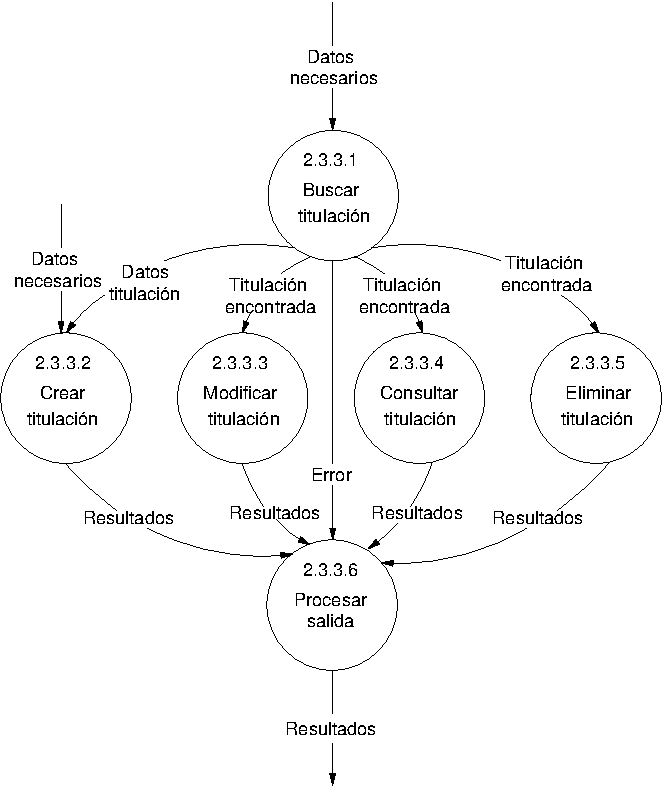
\includegraphics[]{08.Analisis_Funcional/8.2.DFDs/Niveles/Nivel4/AdministradorPrincipal/AdministrarTitulaciones/Diagramas/nivel4-AdministrarTitulaciones.pdf}
      \caption{Nivel de abstracción 4: Administrar titulaciones (módulo Administrador principal).}
      \label{diagramaNivel4-AdministrarTitulaciones}
    \end{center}
  \end{figure}

\paragraph{}En este proceso, el usuario administrador de centro puede crear,
consultar, modificar o borrar asignaturas de la aplicación.

\paragraph{}La figura \ref{diagramaNivel4-AdministrarAsignaturas-admCentro}
muestra el nivel de abstracción 4: Administrar asignaturas (módulo Administrador
de centro).

  \begin{figure}[!ht]
    \begin{center}
      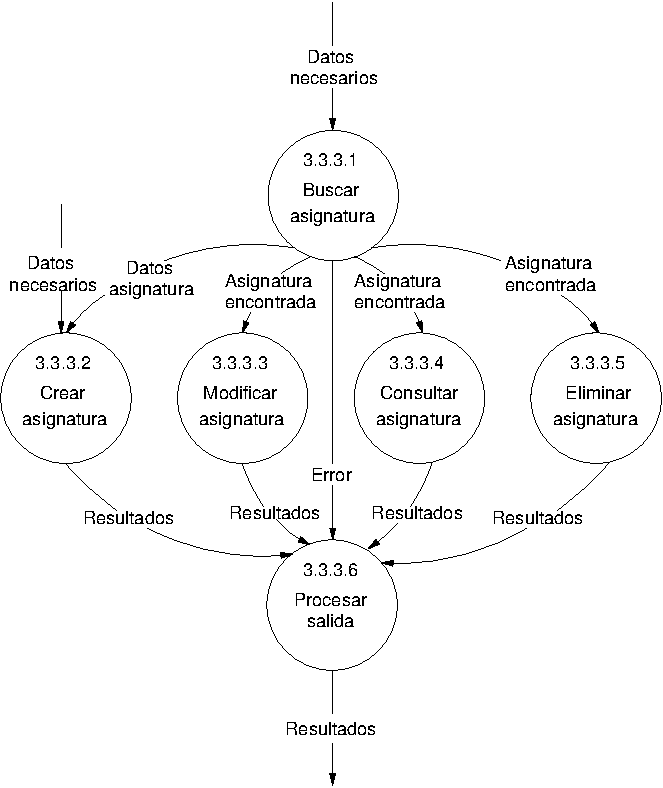
\includegraphics[]{08.Analisis_Funcional/8.2.DFDs/Niveles/Nivel4/AdministradorCentro/AdministrarAsignaturas/Diagramas/nivel4-AdministrarAsignaturas.pdf}
      \caption{Nivel de abstracción 4: Administrar asignaturas (módulo Administrador de centro).}
      \label{diagramaNivel4-AdministrarAsignaturas-admCentro}
    \end{center}
  \end{figure}

\subsection{Administrar usuarios (Módulo Administrador de centro)}

  \paragraph{}El diagrama de la figura
  \ref{diagramaDescomposicionAdministrarUsuarios-admCentro} muestra la
  estructura del módulo Administrar usuarios. Este módulo permitirá al usuario
  administrador de centro realizar el mantenimiento y gestión de la información
  relacionada con los distintos tipos de usuario que formen parte del centro.

  \begin{figure}[!ht]
    \begin{center}
      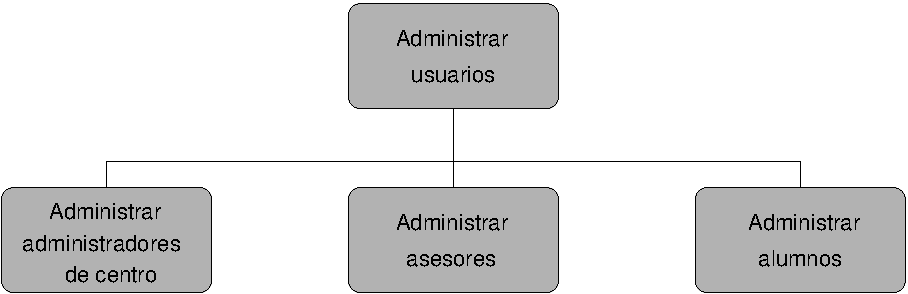
\includegraphics[]{11.Disenyo_Arquitectonico/11.2.Diagramas_Descomposicion/11.2.3.Modulo_administrador_centro/AdministrarBBDD/AdministrarUsuarios/Diagramas/administrar_usuarios.pdf}
      \caption{Diagrama de descomposición Administrar usuarios (módulo Administrador de centro).}
      \label{diagramaDescomposicionAdministrarUsuarios-admCentro}
    \end{center}
  \end{figure}

 \paragraph{}En este proceso, el usuario administrador de centro puede crear,
consultar, modificar o borrar usuarios administradores de centro de la
aplicación.

\paragraph{}La figura \ref{diagramaNivel5-AdministrarAdministradoresCentro-admCentro}
muestra el nivel de abstracción 5: Administrar Administradores de centro (módulo
Administrador de centro).

  \begin{figure}[!ht]
    \begin{center}
      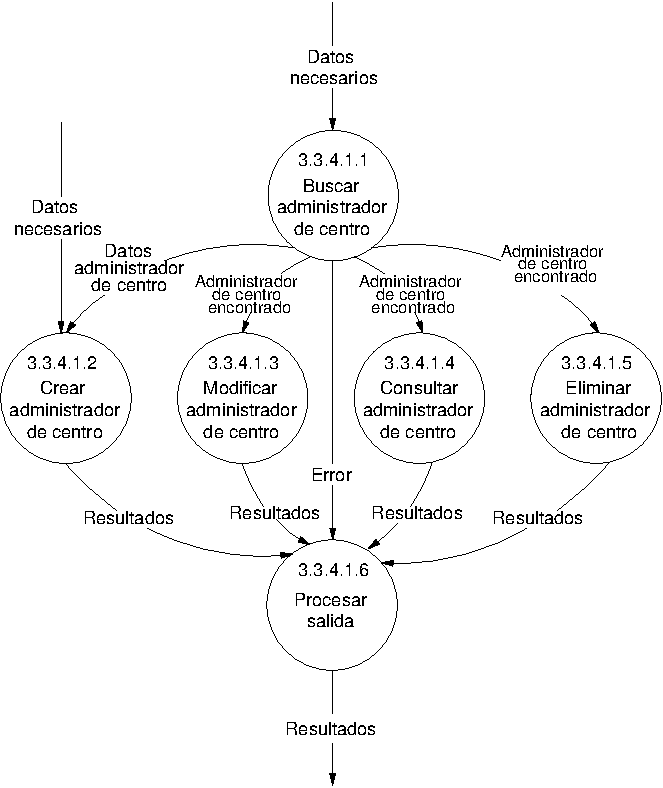
\includegraphics[]{08.Analisis_Funcional/8.2.DFDs/Niveles/Nivel5/AdministradorCentro/AdministrarUsuarios/AdministrarAdministradoresCentro/Diagramas/nivel5-AdministrarAdministradoresCentro.pdf}
      \caption{Nivel de abstracción 5: Administrar Administradores de centro
      (módulo Administrador de centro).}
      \label{diagramaNivel5-AdministrarAdministradoresCentro-admCentro}
    \end{center}
  \end{figure}

 \subsubsection{Administrar Asesores (módulo Administrador de centro)}

  \paragraph{}El diagrama de la figura
  \ref{diagramaDescomposicionAdministrarAsesores-admCentro} muestra la
  estructura del módulo Administrar Asesores. Este módulo permitirá al usuario
  administrador de centro realizar el mantenimiento y gestión de la información
  relacionada con los asesores que formen parte del centro al que pertenece.

  \begin{figure}[!ht]
    \begin{center}
      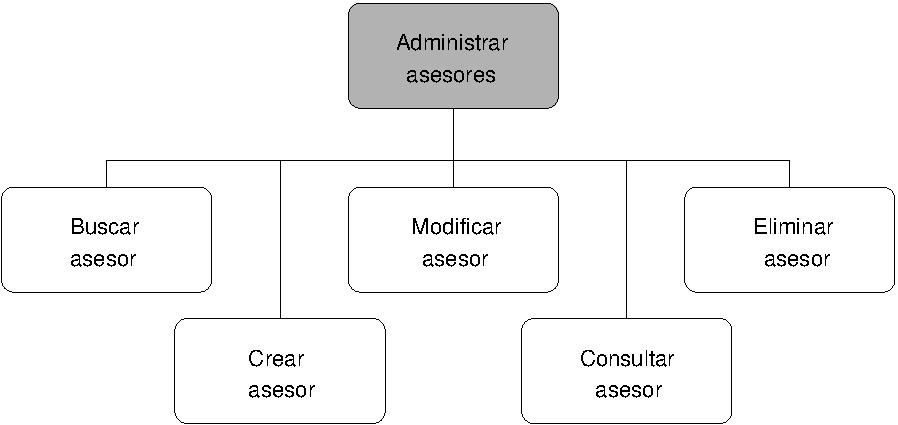
\includegraphics[]{11.Disenyo_Arquitectonico/11.2.Diagramas_Descomposicion/11.2.3.Modulo_administrador_centro/AdministrarBBDD/AdministrarUsuarios/AdministrarAsesores/Diagramas/administrar_asesores.pdf}
      \caption{Diagrama de descomposición Administrar Asesores (módulo Administrador de centro).}
      \label{diagramaDescomposicionAdministrarAsesores-admCentro}
    \end{center}
  \end{figure}

 \subsubsection{Administrar Alumnos (módulo Administrador de centro)}

  \paragraph{}El diagrama de la figura
  \ref{diagramaDescomposicionAdministrarAlumnos-admCentro} muestra la
  estructura del módulo Administrar Alumnos. Este módulo permitirá al usuario
  administrador de centro realizar el mantenimiento y gestión de la información
  relacionada con los alumnos que formen parte del centro al que pertenece.

  \begin{figure}[!ht]
    \begin{center}
      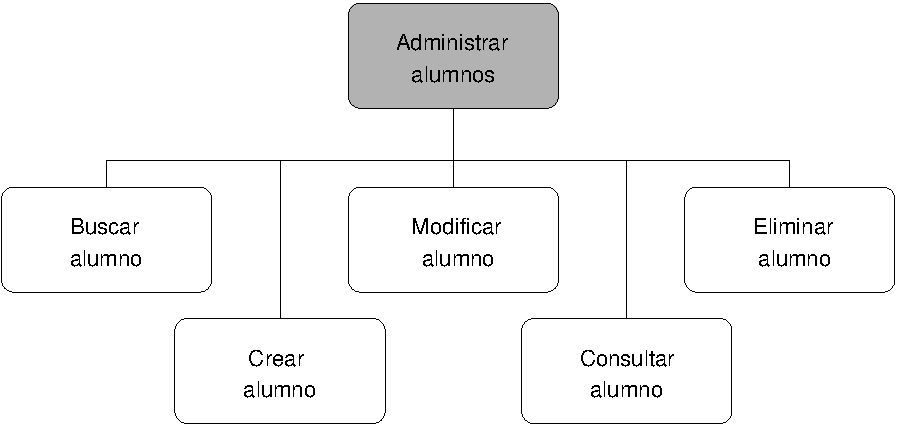
\includegraphics[]{11.Disenyo_Arquitectonico/11.2.Diagramas_Descomposicion/11.2.3.Modulo_administrador_centro/AdministrarBBDD/AdministrarUsuarios/AdministrarAlumnos/Diagramas/administrar_alumnos.pdf}
      \caption{Diagrama de descomposición Administrar Alumnos (módulo Administrador de centro).}
      \label{diagramaDescomposicionAdministrarAlumnos-admCentro}
    \end{center}
  \end{figure}
